\subsection{Photo-multipliers Divider}

In the original readout electronics the LTCC single ouput from each PMT was amplified by a factor of 10
and then splitted in two to feed the ADC and TDC baords. This amplification and splitting was performed
by a dedicated electronic module. 

In 2002 a novel concept \cite{Popov:2003mj} was developed at Jefferson Lab to effectivly amplify a PMT signal by employing a dedicated circuit
to process the anode or dynode signal prior to sending it through a standard 50 $\omega$ line/cable.

The electronic addition to the PMT base provides an additional PMT signal boost while preserving
PMT fast pulse shape. It also improves rate capability. It significantly improves signal amplitude and
signal to noise ratio, which is especially important for low input light signals in cases such as Cherenkov counters.

The design was adapted to use the LTCC XP4500B base and a prototype, shown in \F{pmtWithDivider} was built to provide a x10
amplification and a splitted signal directly from the PMT base.


\begin{figure}
	\centering
	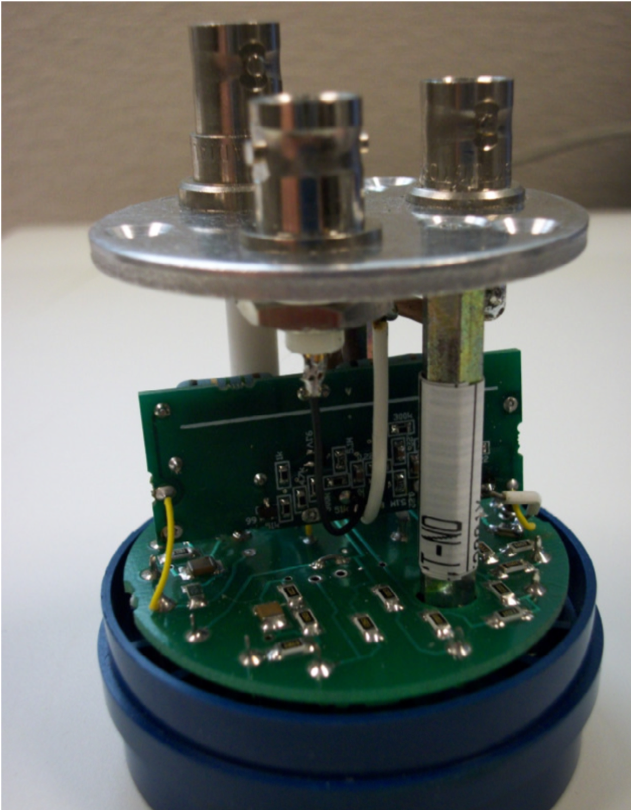
\includegraphics[width=0.95\columnwidth,keepaspectratio]{img/pmtWithDivider.png}
	\caption{The prototype module installed in the XP4500B PMT base. The bottom of the base has been modified to contain the HV
				BNC input and two output signals BNC. }
	\label{fig:pmtWithDivider}
\end{figure}

The following tests were performed successfully:
\begin{itemize}
	\item x10 amplification
	\item splitted signals identity
	\item signal to noise ratio comparison with non modified base
	\item FADC spectrum
\end{itemize}

In \F{dividerTests} the




\begin{figure}
	\centering
	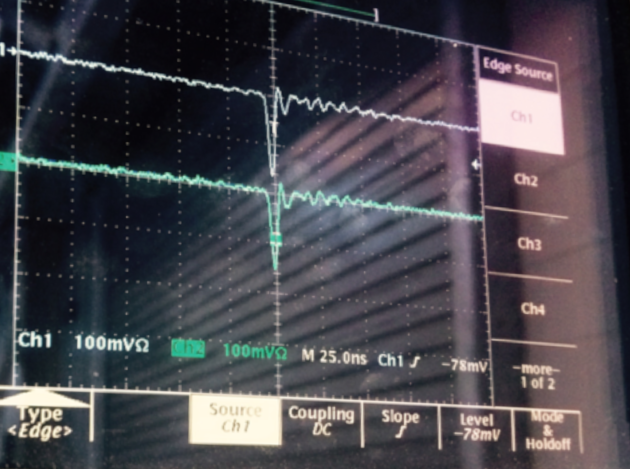
\includegraphics[width=0.87\columnwidth,keepaspectratio]{img/doubleSignal.png}
	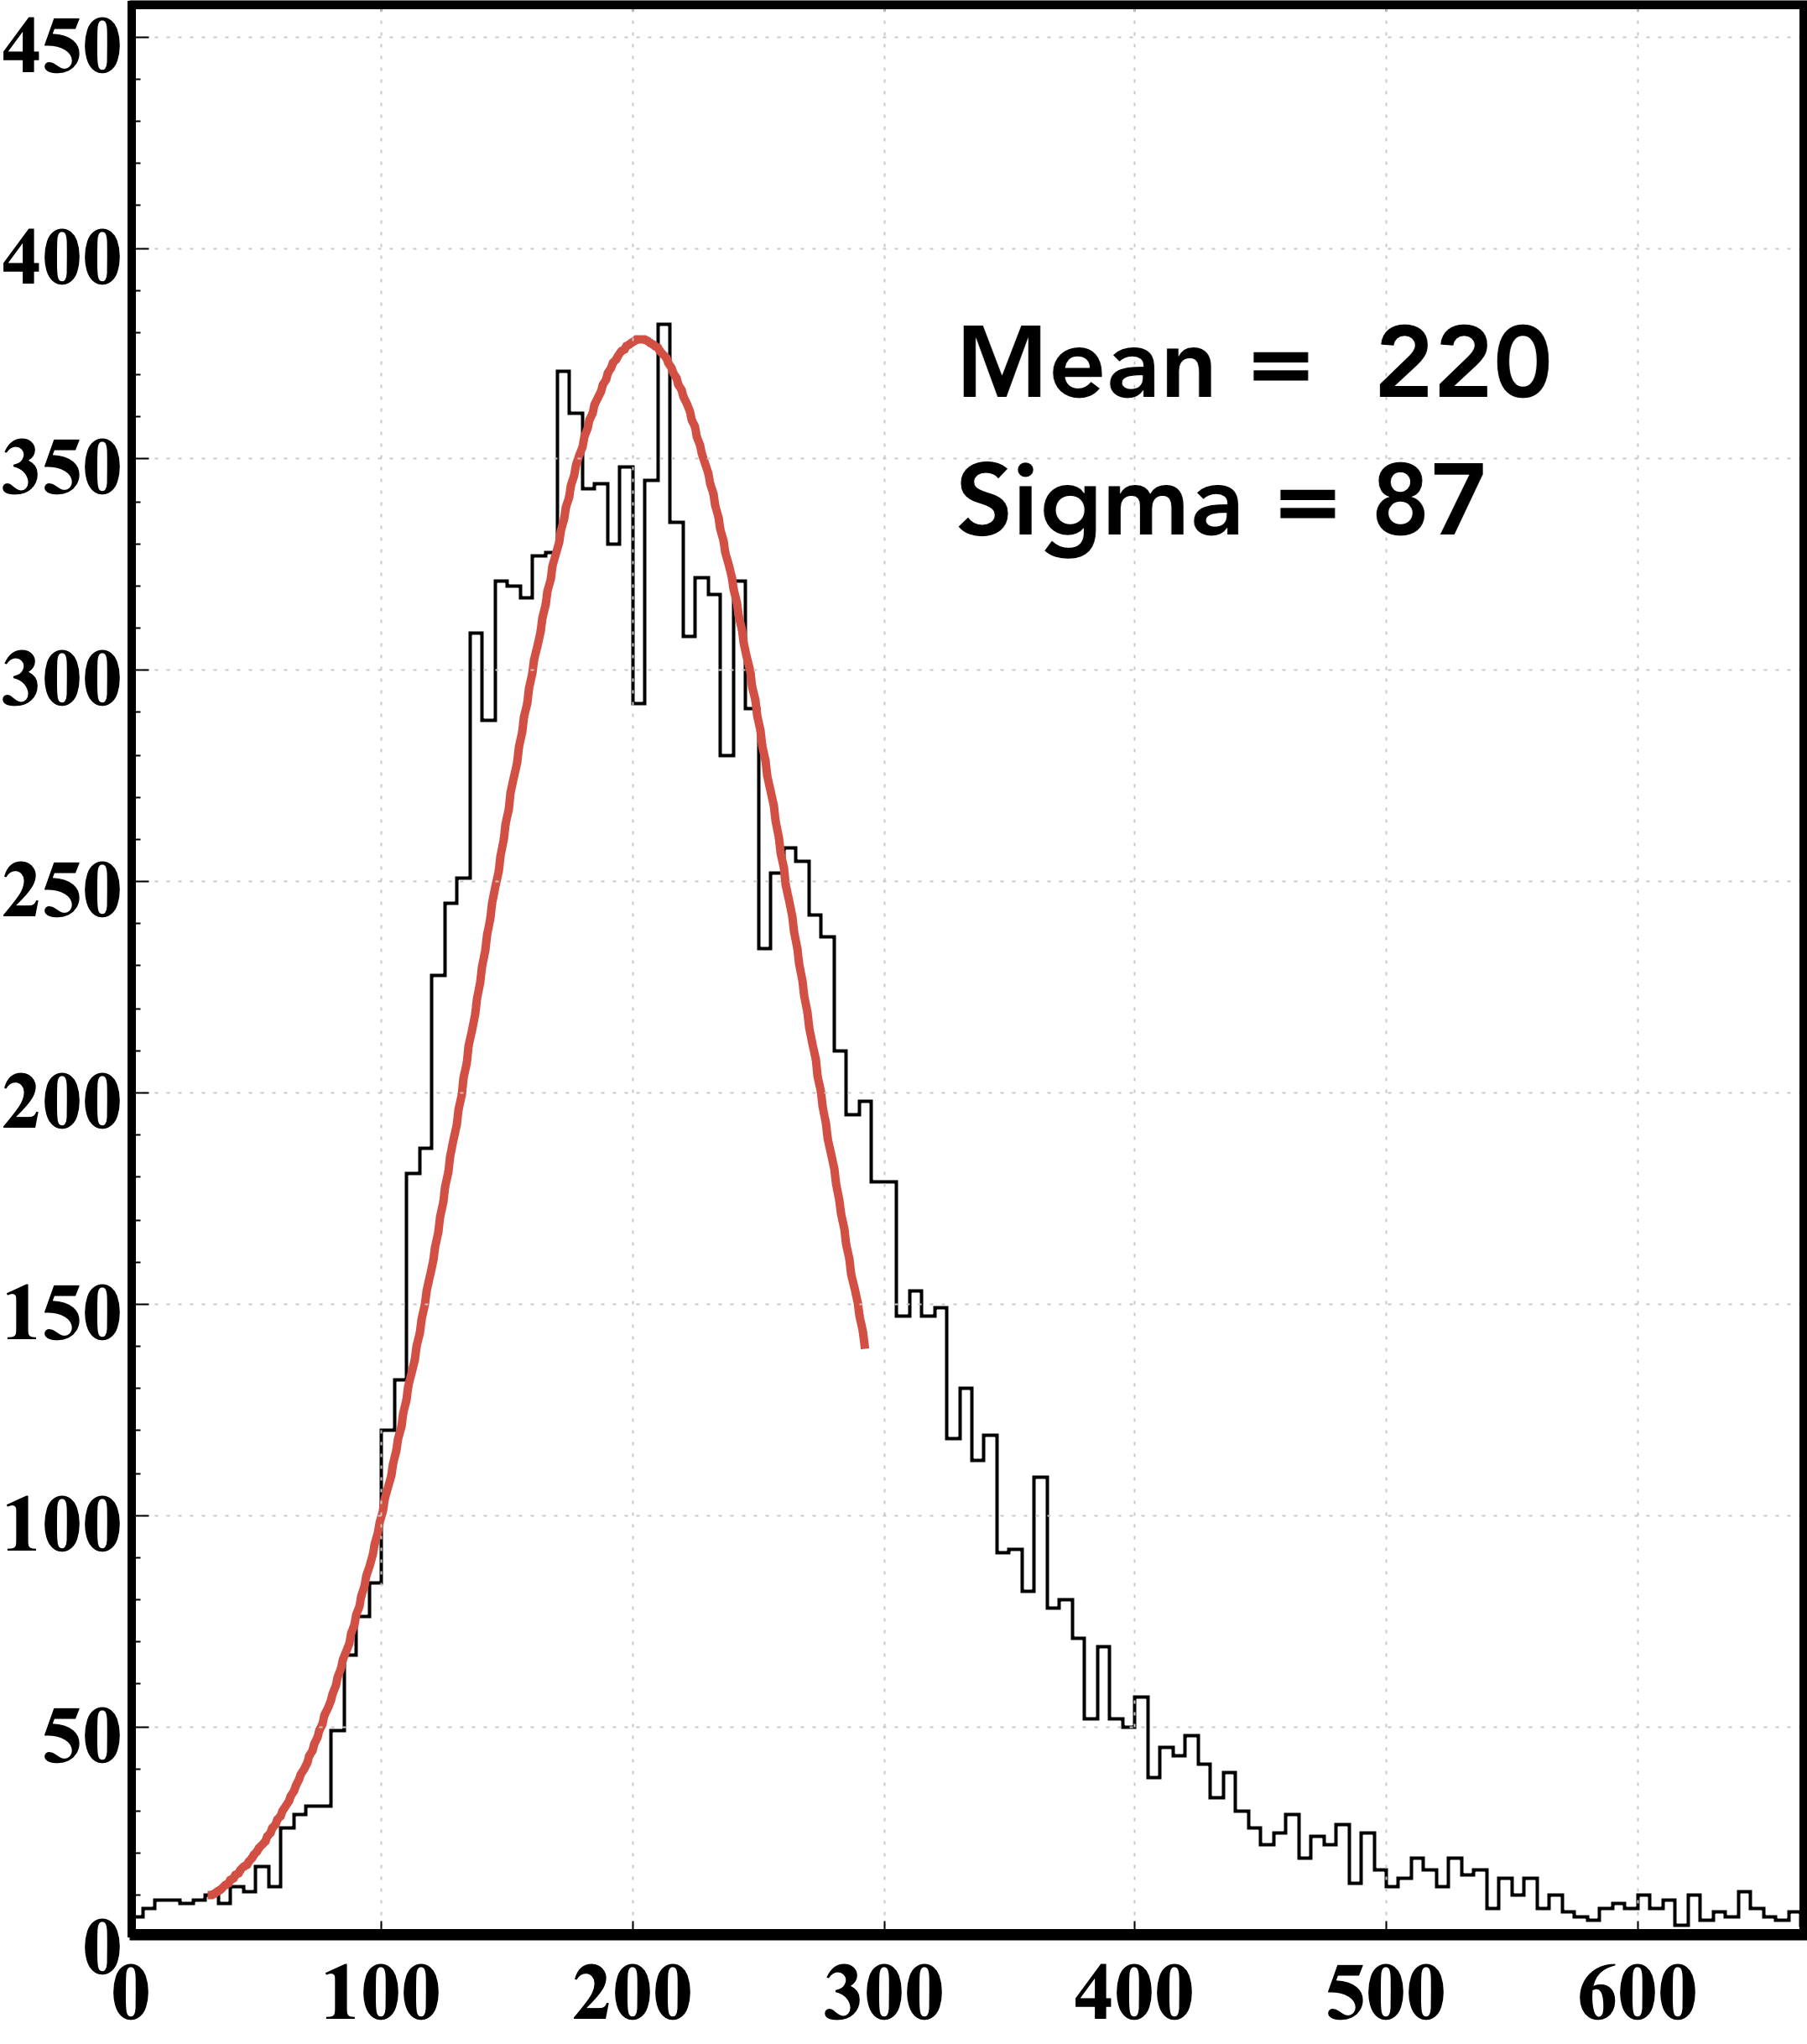
\includegraphics[width=0.97\columnwidth,keepaspectratio]{img/fadcOutput.png}
	\caption{Average number of reflections calculated from simulations studies.}
	\label{fig:dividerTests}
\end{figure}

dsg work

final implementation: 200 modules

